
\chapter{Matching in  Observational Studies}\label{chapter::matching-obs}
 
Matching has a long history in empirical research. W. Cochran and D. Rubin popularized it in statistical causal inference.   \citet{cochran1973controlling} is an early review paper. \citet{rubin2006matched} collects Rubin's contributions to this topic. 
This chapter also discusses modern contributions by \citet{abadie2006large, abadie2008failure, abadie2011bias} based on the asymptotic analysis of matching estimators. 

 

\section{A simple starting point: many more control units}
\label{sec::ideal-matching-mpe}

\begin{figure}[ht]
\centering 
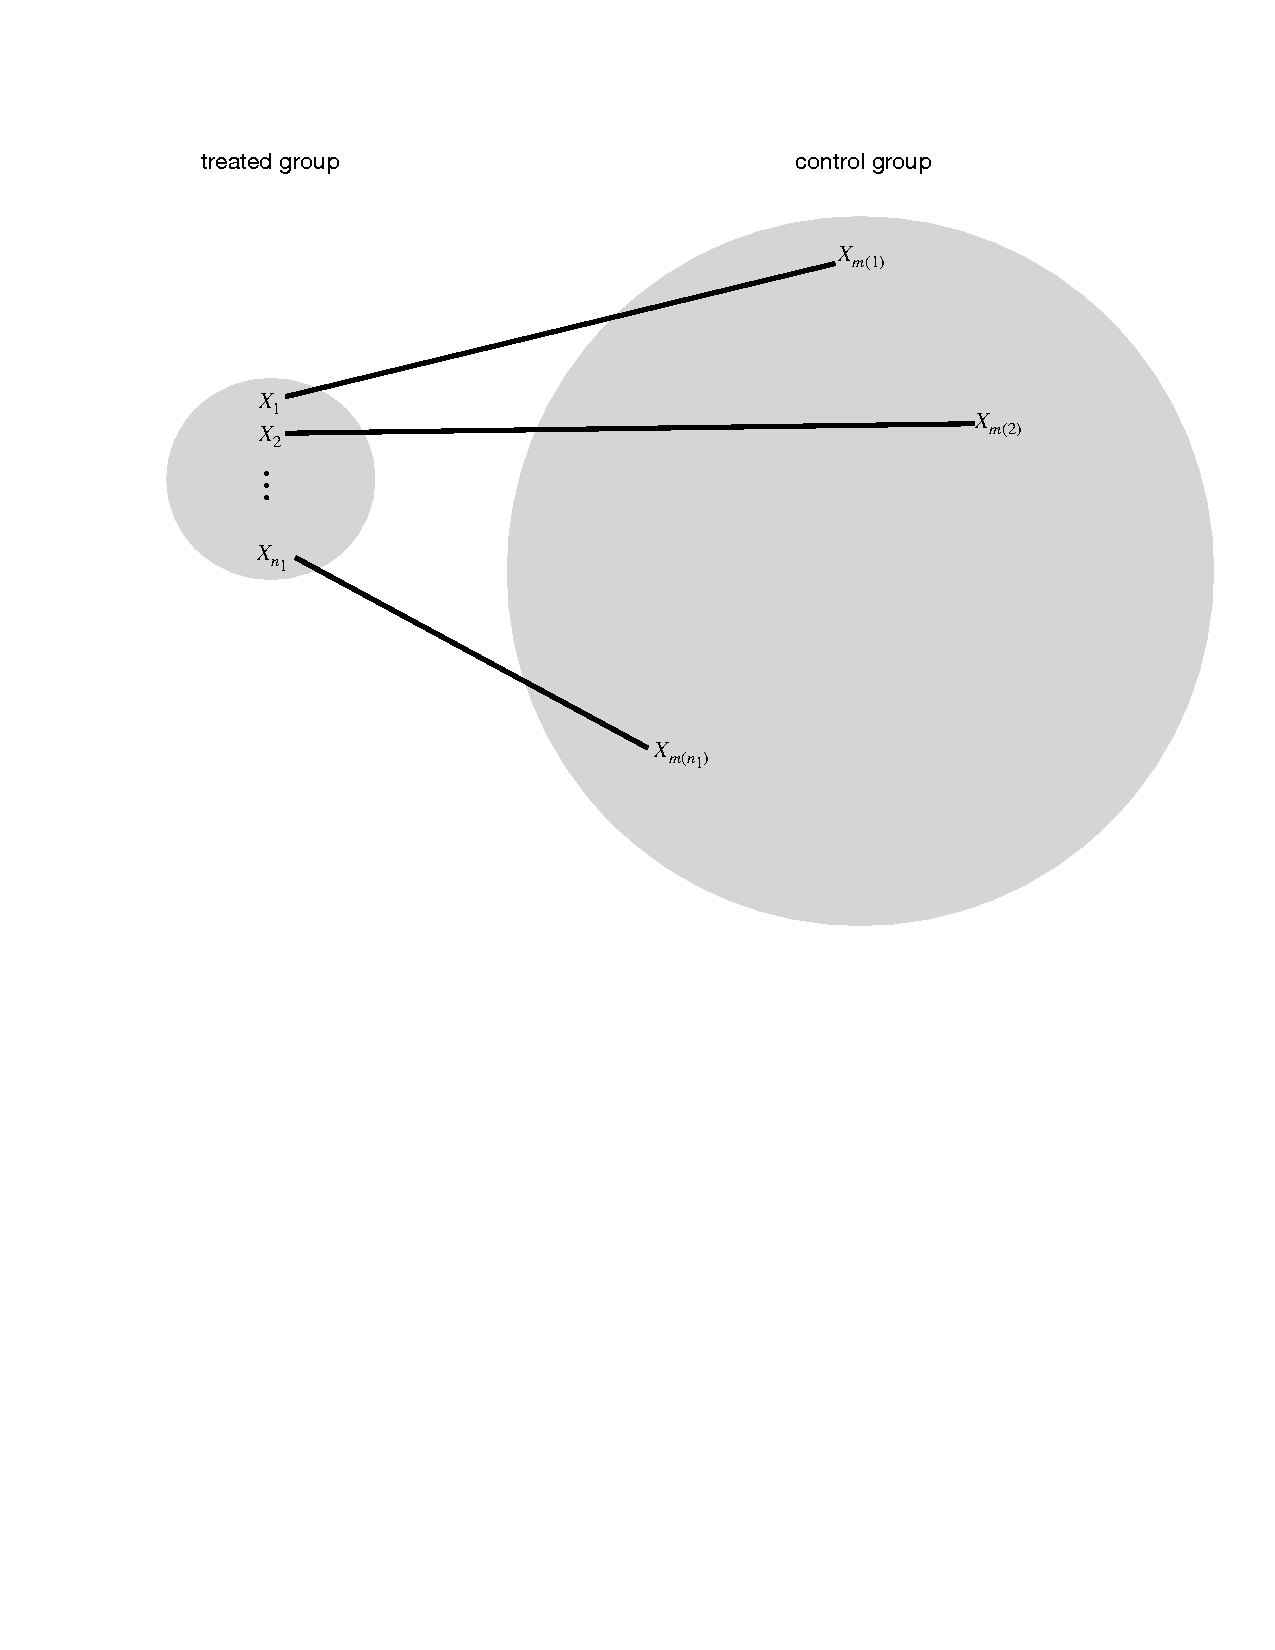
\includegraphics[width = \textwidth]{figures/matchingonetoone.pdf}
\caption{Illustration of matching in observational studies}\label{fig::matching-causal}
\end{figure}


Figure \ref{fig::matching-causal} illustrates the basic idea of matching in treatment-control observational studies. 
Consider a simple case with the number of control units $n_0$ being much larger than the number of treated units $ n_1$. For unit $i=1,\ldots, n_1$ in the treated group, we find a unit $m(i)$ in the control group such that $X_i = X_{m(i)}$. In the ideal case, we have exact matches. Therefore, the units within a matched pair have the same propensity score $e(X_i) = e(X_{m(i)})$. Consequently, conditional on the event that one unit receives the treatment and the other receives the control, the probability of unit $i$ receiving the treatment and unit $m(i)$ receiving the control is
$$
\pr( Z_i = 1, Z_{m(i)} = 0 \mid  Z_i +Z_{m(i)} = 1, X_i, X_{m(i)} )  = 1/2
$$
by a symmetry argument.\footnote{The rigorous argument is
\begin{eqnarray*}
&&\pr( Z_i = 1, Z_{m(i)} = 0 \mid  Z_i +Z_{m(i)} = 1, X_i, X_{m(i)} ) \\
&=& \frac{ \pr( Z_i = 1, Z_{m(i)} = 0 \mid   X_i, X_{m(i)} ) }{ \pr( Z_i = 1, Z_{m(i)} = 0 \mid   X_i, X_{m(i)} )   + \pr( Z_i = 0, Z_{m(i)} = 1 \mid   X_i, X_{m(i)} ) } \\
&=& \frac{  e(X_i)  \{ 1 - e(X_{m(i)}) \}  }{ e(X_i)  \{ 1 - e(X_{m(i)}) \}   + \{1-e(X_i)\} e(X_{m(i)}) } \\
&=& \frac{1}{2}.
\end{eqnarray*}
}
That is, the treatment assignment is identical to the MPE conditioning on the covariates and the event that each pair has a treated unit and a control unit. So we can analyze the exactly matched observational study as if it is an MPE, using either the FRT or the Neymanian approach in Chapter \ref{chapter::mpe}. This gives us inference on the causal effect on the treated units. 


We can also find multiple control units for each treated unit. In general, we can find $M_i$ matched control units for the treated unit $i$. When the $M_i$'s vary, it is called the {\it variable-ratio matching} \citep{ming2000substantial, ming2001note, pimentel2015variable}. With perfect matching, the treatment assignment mechanism is identical to the general matched experiment discussed in Section \ref{sec::general-matched-experiment}. We can use the analytic results in that section to analyze the matched observational study. 


\citet{rosenbaum2002design} advocated the above analysis strategy. In most observational studies, however, $X_i = X_{m(i)}$ does not hold for all units. The above reasoning for FRT does not hold.  Recently, \citet{guo2022statistical} reported negative results on the consequence of inexact matching in FRT. This is a warning of this strategy. 
 


\section{A more complicated but realistic scenario}

Even if the control group is large, we often do not have exact matches. What we can achieve is that $X_i \approx X_{m(i)}  $ or $X_i -X_{m(i)} $ is small under some distance metric. So we have only approximate matches. For example, we define
$$
m(i) = \arg\min_{k:Z_k = 0} d(X_i ,X_k), 
$$
where $d(X_i ,X_k)$ measures the distance between $X_i$ and $X_k$. Some canonical choices of the distance are the Euclidean distance
$$
d(X_i ,X_k) =  (X_i - X_k)\tran ( X_i - X_k),
$$
and the Mahalanobis distance
%\footnote{We define $\|v\|_2^2 = \sum_{j=1}^p v_j^2$ for a vector $v = (v_1, \ldots, v_p)\tran$. It denotes the squared length of the vector $v$.}
$$
d(X_i ,X_k) =(X_i - X_k)\tran \Omega^{-1} (X_i - X_k)
$$
with $\Omega$ being the sample covariance matrix of the $X_i$'s from the whole population or only the control group. 


I review some subtle issues about matching below. See \citet{stuart2010matching} for a review paper. 
\begin{enumerate}
\item
(one-to-one or one-to-$M$ matching)
The above discussion focused on one-to-one matching. We can also extend the discussion to one-to-$M$ matching.


\item
I focus on matching with replacement but some practitioners prefer matching without replacement. If the pool of control units is large, these two methods will not differ too much for the final result. Matching with replacement is computationally more convenient, but matching without replacement involves computationally intensive discrete optimization. Matching with replacement usually gives matches of higher quality but it introduces dependence by using the same units multiple times. In contrast, the advantage of matching without replacement is the independence of matched units and the simplicity in the subsequent data analysis. 


\item
Because of the residual covariate imbalance within matched pairs, it is crucial to use covariate adjustment when analyzing the data. In this case, covariate adjustment is not only for efficiency gain but also for bias correction.

\item
If $X$ is ``high dimensional'', it is likely that $d(X_i ,X_k)$ is too large for some unit $i$ in the treated group and for all choices of the units in the control group. If this happens, we may have to drop some units that are hard to find matches. By doing this, we effectively change the study population of interest.  


\item
It is hard to avoid the above problem. For example, if $X_i \sim \text{N}(0, I_p), X_k \sim\text{N}(0, I_p) ,$ and $X_i \ind X_k$, then 
$$
(X_i - X_k)\tran (X_i - X_k) \sim    2 \chi^2_p
$$ 
which has mean $2p$ and variance $8p$ (see Chapter \ref{subsection::chi2-t-distribution}). 
Theory shows that with large $p$, imperfect matching causes a large bias in causal effect estimation. 
This suggests that if $p$ is large,  we must do some dimension reduction before matching. 
\citet{rosenbaum1983central} proposed to use matching based on the propensity score. With the estimated propensity score, we find pairs of units $\{ i, m(i)\}$ with small values of $ |  \hat{e}(X_i) -  \hat{e}(X_{m(i)})  |$ or $| \logit\{ \hat{e}(X_i)\} - \logit\{ \hat{e}(X_{m(i)}) \} | $\footnote{Define $\logit(w) = \log \frac{w}{1-w}$. The logit function is a map from $[0,1]$ to $(-\infty, \infty)$.}, i.e., we have a one-dimensional matching problem. 
\end{enumerate}

 

\section{Matching estimator for the average causal effect}

In a sequence of papers, Abadie and Imbens (AI) rigorously characterized the asymptotic properties of the matching estimator and proposed the corresponding large-sample confidence intervals for the average causal effect. 
They chose the standard setup for observational studies with  $\{ X_i , Z_i ,Y_i(1), Y_i(0)  \}_{i=1}^n \iidsim \{ X, Z, Y(1), Y(0) \}$.  

\subsection{Point estimation and bias correction}

AI focused on $1$-$M$ matching with replacement. For a treated unit $i$, we can simply impute the potential outcome under the treatment as $\hat{Y}_i(1) = Y_i$, and impute the potential outcome under the control as 
$$
\hat{Y}_i(0) = M^{-1} \sum_{k\in J_i} Y_k,
$$
where $J_i$ is the set of matched units from the control group for unit $i$. For example, we can compute $d(X_i, X_k)$ for all $k$ in the control group, and then define $J_i$ as the indices of $k$ with the $M$ smallest values of $d(X_i, X_k)$. 




For a control unit $i$, we simply impute the potential outcome under the control as $\hat{Y}_i(0) = Y_i$, and impute the potential outcome under the treatment as
$$
\hat{Y}_i(1) = M^{-1} \sum_{k\in J_i} Y_k,
$$
where $J_i$ is the set of matched units from the treatment group for unit $i$.

The matching estimator is 
$$
\hat{\tau}^\textup{m} = n^{-1} \sumn \{\hat{Y}_i(1) -\hat{Y}_i(0) \}.
$$

AI showed that $\hat{\tau}^\textup{m}$ has non-negligible bias especially when $X$ is multidimensional and the number of control units is comparable to the number of treated units. Through some technical derivations,  they proposed the following estimator for the bias: 
$$
\hat{B} = n^{-1} \sumn  \hat{B}_i
$$
where
$$
\hat{B}_i = (2Z_i - 1) M^{-1} \sum_{k\in J_i} \{  \hat{\mu}_{1-Z_i}(X_i) -  \hat{\mu}_{1-Z_i}(X_k)     \}
$$
with $\{  \hat{\mu}_1(X_i), \hat{\mu}_0(X_i) \}$ being the predicted outcomes by, for example, OLS fits. 
For a treated unit with $Z_i  =1$, the estimated bias is
$$
\hat{B}_i = M^{-1} \sum_{k\in J_i} \{  \hat{\mu}_{0}(X_i) -  \hat{\mu}_{0}(X_k)     \}
$$
which corrects the discrepancy in predicted control potential outcomes due to the mismatch in covariates; for a control unit with $Z_i = 0$, the estimated bias is
 $$
\hat{B}_i =  - M^{-1} \sum_{k\in J_i} \{  \hat{\mu}_{1}(X_i) -  \hat{\mu}_{1}(X_k)     \}
$$
which corrects the discrepancy in predicted treated potential outcomes due to the mismatch in covariates. 


The final bias-corrected matching estimator is
$$
\hat{\tau}^\textup{mbc} = \hat{\tau}^\textup{m}  - \hat{B},
$$
 which has the following linear expansion.
 
 \begin{proposition}
 \label{prop::matching-expansion-ate} We have 
 \begin{eqnarray}\label{eq::linearATE}
\hat{\tau}^\textup{mbc}  
= n^{-1} \sumn \hat{\psi}_i
\end{eqnarray} 
where 
 $$
  \hat{\psi}_i = \hat{\mu}_1(X_i) -  \hat{\mu}_0(X_i) + (2Z_i - 1) (1+K_i/M) \{   Y_i - \hat{\mu}_{Z_i}(X_i)  \}
 $$
 with $K_i$ being the times that unit $i$ is used as a match. 
 \end{proposition}
 
 
 
The linear expansion in Proposition  \ref{prop::matching-expansion-ate} follows from simple but tedious algebra. I leave its proof as Problem \ref{para::linear-bcm-ate}. The linear expansion motivates a simple variance estimator 
$$
\hat{V}^\textup{mbc}  = \frac{1}{n^2} \sumn (  \hat{\psi}_i - \hat{\tau}^\textup{mbc}  )^2,
$$
by viewing $\hat{\tau}^\textup{mbc}  $ as sample averages of the $  \hat{\psi}_i $'s.  \citet{abadie2008failure}  first showed that the simple bootstrap by resampling the original data does not work for estimating the variance of the matching estimators, but their proposed variance estimation procedure is not easy to implement.  \citet{otsu2017bootstrap} proposed to bootstrap the $  \hat{\psi}_i $'s in the linear expansion. However,  \citet{otsu2017bootstrap}'s bootstrap essentially yields the variance estimator $\hat{V}^\textup{mbc}  $, which is simple to calculate. 


 
\subsection{Connection with the doubly robust estimators}
 \label{sec::connection-dr-att}
 
The bias-corrected matching estimators and the doubly robust estimators are closely related. They both equal the outcome regression estimator
with some modifications based on the residuals 
$$ 
 \hat{R}_i = 
 \begin{cases}
 Y_i - \hat{\mu}_1(X_i)  & \text{ if } Z_i=1;\\
 Y_i - \hat{\mu}_0(X_i)    & \text{ if } Z_i=0.
\end{cases} 
 $$
  For the average causal effect $\tau$, recall the outcome regression estimator  
$$
\hat{\tau}^{\textup{reg}} =  n^{-1} \sumn \{ \hat{\mu}_1(X_i) -  \hat{\mu}_0(X_i)\} 
$$
and the doubly robust estimator 
$$
\hat{\tau}^\textup{dr}  =  \hat{\tau}^{\textup{reg}} 
+ n^{-1} \sumn \left\{  \frac{Z_i \hat{R}_i }{ \hat{e}(X_i)} -  \frac{ (1-Z_i) \hat{R}_i}{ 1-  \hat{e}(X_i) } \right\} .
$$
Furthermore, we can verify that $\hat{\tau}^\textup{mbc} $ has a form similar to $\hat{\tau}^\textup{dr}  $.
\begin{proposition}
\label{prop::mbc-dr}
The bias-corrected matching estimator for $\tau$ equals 
$$
\hat{\tau}^\textup{mbc}   =\hat{\tau}^{\textup{reg}} 
+ n^{-1} \sumn \left\{ \left(1+{ K_i\over M} \right)  Z_i \hat{R}_i  - \left( 1+{ K_i\over M} \right) (1-Z_i)  \hat{R}_i \right\} .
$$
\end{proposition}

I leave the proof of Proposition \ref{prop::mbc-dr}  as Problem \ref{para::dr-mbc-form}.  From Proposition \ref{prop::mbc-dr}, we can view matching as a nonparametric method to estimate the propensity score, and the resulting bias-corrected matching estimator as a doubly robust estimator. For instance, $1+K_i /  M$ should be close to $1/\hat{e}(X_i)$. When a treated unit has a small $e(X_i)$, the resulting weight based on the estimated propensity score $1/\hat{e}(X_i)$ will be large, and at the same time, it will be matched to many control units, resulting in large $K_i$ and thus large $1+K_i /  M$. However, this connection also raised an obvious question regarding matching. With a fixed $M$, the estimator $1+K_i /  M$ for $1/e(X_i)$ will be very noisy. Allowing $M$ to grow with the sampling size is likely to improve the matching-based nonparametric estimator for the propensity score and thus improve the asymptotic properties of the matching and bias-corrected matching estimators. \citet{lin2023estimation} provided a formal theory that once we allow $M$ to grow at a proper rate, the bias-corrected matching estimator $\hat{\tau}^\textup{mbc}   $ can achieve similar properties as the doubly robust estimator.  


 
 
 \section{Matching estimator for the average causal effect on the treated}

 
For the average causal effect on the treated 
$$
\tau_\textsc{T} = E(Y\mid Z=1) - E\{  Y(0)  \mid Z=1\},
$$ 
we only need to impute the missing potential outcomes under control for all the treated units, resulting in the following estimator
$$
\hat{\tau}_\textsc{T}^\textup{m} = n_1^{-1} \sumn Z_i \{  Y_i - \hat{Y}_i(0) \}.
$$
Again it is biased with multidimensional $X$.
\citet{otsu2017bootstrap} propose to estimate its bias by 
$$  
\hat{B}_\textsc{T} = n_1^{-1} \sumn Z_i  \hat{B}_{\textsc{T},i} 
$$
where
$$
\hat{B}_{\textsc{T},i} = M^{-1} \sum_{k \in J_i} \{  \hat{\mu}_0(X_i) -  \hat{\mu}_0(X_k)     \}
$$
corrects the bias due to the mismatch of covariates for a treated unit with $Z_i = 1.$


The final bias-corrected estimator is
$$
\hat{\tau}_\textsc{T}^\textup{mbc} = \hat{\tau}_\textsc{T}^\textup{m} - \hat{B}_\textsc{T},
$$ 
which has the following linear expansion.

\begin{proposition}\label{prop::linear-expansion-att}
We have 
\begin{eqnarray}\label{eq::linearATT}
\hat{\tau}_\textsc{T}^\textup{mbc}  =   n_1^{-1} \sumn \hat{\psi}_{\textsc{T}, i},
\end{eqnarray}
where 
$$
\hat{\psi}_{\textsc{T}, i} =   Z_i \{ Y_i - \hat{\mu}_0(X_i) \}
- (1-Z_i) K_i/M \{ Y_i - \hat{\mu}_0(X_i) \} . 
$$
\end{proposition}

I leave the proof to Problem \ref{para::linear-bcm-ate}. 
Motivated by \citet{otsu2017bootstrap}, we can view $\hat{\tau}_\textsc{T}^\textup{mbc}  $ as $n/n_1$ multiplied by the sample average of the $\hat{\psi}_{\textsc{T}, i}$'s, so an intuitive variance estimator is
$$
\hat{V}_\textsc{T}^\textup{mbc} =  \left( \frac{n}{n_1} \right)^2 \frac{1}{n^2} \sumn (\hat{\psi}_{\textsc{T}, i} - \hat{\tau}_\textsc{T}^\textup{mbc} n_1/n)^2 = \frac{1}{n_1^2} \sumn (\hat{\psi}_{\textsc{T}, i} - \hat{\tau}_\textsc{T}^\textup{mbc} n_1/n )^2.
$$

 
 Similar to the discussion in Section \ref{sec::connection-dr-att}, we can compare the doubly robust and bias-corrected matching estimators with the outcome regression estimator. 
 For the average causal effect on the treated units $\tau_\textsc{T}$, recall the outcome regression estimator 
$$
\hat{\tau}^{\textup{reg}}_\textsc{T} = n_1^{-1} \sumn Z_i \{ Y_i - \hat{\mu}_0(X_i) \} ,
$$
and the doubly robust estimator
$$
\hat{\tau}_\textsc{T}^\textup{dr} =  \hat{\tau}^{\textup{reg}}_\textsc{T} 
- n_1^{-1} \sumn \frac{  \hat{e}(X_i) }{ 1- \hat{e}(X_i) }  (1-Z_i)  \hat{R}_i .
$$
Furthermore, we can verify that $\hat{\tau}_\textsc{T}^\textup{mbc} $ has a form similar to $\hat{\tau}_\textsc{T}^\textup{dr} $. 
\begin{proposition}
\label{prop::mbc-dr-att}
The bias correction matching estimator for  $\tau_\textsc{T}$ equals
$$
\hat{\tau}_\textsc{T}^\textup{mbc}   = \hat{\tau}^{\textup{reg}}_\textsc{T} 
 - n_1^{-1} \sumn { K_i\over M}  (1-Z_i)  \hat{R}_i.
$$
\end{proposition}


I leave the proof of Proposition \ref{prop::mbc-dr-att}  as Problem \ref{para::dr-mbc-form-att}.  Proposition \ref{prop::mbc-dr-att} suggests that matching essentially uses $K_i/M$ to estimate the odds of the treatment given covariates. 




\section{A case study}
\label{sec::matching-application}



\subsection{Experimental data}
Now I revisit the LaLonde data using \citet{sekhon2011multivariate}'s \ri{Matching} package. We have used this package several times for the dataset \ri{lalonde}, and now we will use its key function \ri{Match}.  The experimental part gives us the following results:
\begin{lstlisting}
> library("car")
> library("Matching")
> 
> ## Chapter 15.5.1
> ## experimental data
> data("lalonde")
> y = lalonde$re78
> z = lalonde$treat
> x = as.matrix(lalonde[, c("age", "educ", "black",
+                           "hisp", "married", "nodegr",
+                           "re74", "re75")])
> 
> ## analysis the randomized experiment
> neymanols = lm(y ~ z)
> fisherols = lm(y ~ z + x)
> xc = scale(x)
> linols = lm(y ~ z*xc)
> resols = c(neymanols$coef[2],
+            fisherols$coef[2],
+            linols$coef[2],
+            sqrt(hccm(neymanols, type = "hc2")[2, 2]),
+            sqrt(hccm(fisherols, type = "hc2")[2, 2]),
+            sqrt(hccm(linols, type = "hc2")[2, 2]))
> resols = matrix(resols, 3, 2)
> rownames(resols) = c("neyman", "fisher", "lin")
> colnames(resols) = c("est", "se")
> resols 
            est       se
neyman 1794.343 670.9967
fisher 1676.343 677.0493
lin    1621.584 694.7217
\end{lstlisting} 
All regression estimators show positive significant results on the job training program. We can analyze the data as if it is an observational study based on 1-1 matching, yielding the following results:
\begin{lstlisting}
> matchest.adj = Match(Y = y, Tr = z, X = x, BiasAdjust = TRUE)
> summary(matchest.adj)

Estimate...  2119.7 
AI SE......  876.42 
T-stat.....  2.4185 
p.val......  0.015583 

Original number of observations..............  445 
Original number of treated obs...............  185 
Matched number of observations...............  185 
Matched number of observations  (unweighted).  268
\end{lstlisting} 
Both the point estimator and standard error increase, but qualitatively, the conclusion remains the same. 


\subsection{Observational data}
Then I revisit the observational counterpart of the data:
\begin{lstlisting}
> dat <- read.table("cps1re74.csv", header = TRUE)
> dat$u74 <- as.numeric(dat$re74==0)
> dat$u75 <- as.numeric(dat$re75==0)
> y = dat$re78
> z = dat$treat
> x = as.matrix(dat[, c("age", "educ", "black",
+                           "hispan", "married", "nodegree",
+                           "re74", "re75", "u74", "u75")])
 \end{lstlisting} 
If we use simple OLS estimators, the results are far from the experimental benchmark and are sensitive to the specification of the regression:
\begin{lstlisting}
> neymanols = lm(y ~ z)
> fisherols = lm(y ~ z + x)
> xc = scale(x)
> linols = lm(y ~ z*xc)
> resols = c(neymanols$coef[2],
+            fisherols$coef[2],
+            linols$coef[2],
+            sqrt(hccm(neymanols, type = "hc2")[2, 2]),
+            sqrt(hccm(fisherols, type = "hc2")[2, 2]),
+            sqrt(hccm(linols, type = "hc2")[2, 2]))
> resols = matrix(resols, 3, 2)
> rownames(resols) = c("neyman", "fisher", "lin")
> colnames(resols) = c("est", "se")
> resols 
             est        se
neyman -8506.495  583.4426
fisher  1067.546  628.4389
lin    -4265.801 3211.7718
  \end{lstlisting} 
  However, if we use 1-1 matching, the results almost recover those based on the experimental data:
  \begin{lstlisting}
> matchest = Match(Y = y, Tr = z, X = x, BiasAdjust = TRUE)
> summary(matchest)

Estimate...  1747.8 
AI SE......  916.59 
T-stat.....  1.9068 
p.val......  0.056543 

Original number of observations..............  16177 
Original number of treated obs...............  185 
Matched number of observations...............  185 
Matched number of observations  (unweighted).  248
   \end{lstlisting} 
   
Ignoring the ties in the matched data, we can also use the matched-pairs analysis, which again yields results similar to those based    on the experimental data:
  \begin{lstlisting}
> diff = y[matchest$index.treated] - 
+           y[matchest$index.control]
> round(summary(lm(diff ~ 1))$coef[1, ], 2)
  Estimate Std. Error    t value   Pr(>|t|) 
   1581.44     558.55       2.83       0.01 
> 
> diff.x = x[matchest$index.treated, ] - 
+               x[matchest$index.control, ]
> round(summary(lm(diff ~ diff.x))$coef[1, ], 2)
  Estimate Std. Error    t value   Pr(>|t|) 
   1842.06     578.37       3.18       0.00 
   \end{lstlisting} 
   
   
   
   \subsection{Covariate balance checks}
   
Moreover, we can use simple OLS to check covariate balance. Before matching, the covariates are highly imbalanced, signified by many stars associated with the coefficients. 
  \begin{lstlisting}
> lm.before = lm(z ~ x)
> summary(lm.before) 

Residuals:
     Min       1Q   Median       3Q      Max 
-0.18508 -0.01057  0.00303  0.01018  1.01355 

Coefficients:
              Estimate Std. Error t value Pr(>|t|)    
(Intercept)  1.404e-03  6.326e-03   0.222   0.8243    
xage        -4.043e-04  8.512e-05  -4.750 2.05e-06 ***
xeduc        3.220e-04  4.073e-04   0.790   0.4293    
xblack       1.070e-01  2.902e-03  36.871  < 2e-16 ***
xhispan      6.377e-03  3.103e-03   2.055   0.0399 *  
xmarried    -1.525e-02  2.023e-03  -7.537 5.06e-14 ***
xnodegree    1.345e-02  2.523e-03   5.331 9.89e-08 ***
xre74        7.601e-07  1.806e-07   4.208 2.59e-05 ***
xre75       -1.231e-07  1.829e-07  -0.673   0.5011    
xu74         4.224e-02  3.271e-03  12.914  < 2e-16 ***
xu75         2.424e-02  3.399e-03   7.133 1.02e-12 *** 
      \end{lstlisting} 
      
      
      However, after matching, the covariates are well-balanced, signified by the absence of stars for all coefficients. 
      
      
   \begin{lstlisting}
> lm.after = lm(z ~ x, 
+               subset = c(matchest$index.treated, 
+                          matchest$index.control))
> summary(lm.after) 

Residuals:
     Min       1Q   Median       3Q      Max 
-0.66864 -0.49161 -0.03679  0.50378  0.65122 

Coefficients:
              Estimate Std. Error t value Pr(>|t|)  
(Intercept)  6.003e-01  2.427e-01   2.474   0.0137 *
xage         3.199e-03  3.427e-03   0.933   0.3511  
xeduc       -1.501e-02  1.634e-02  -0.918   0.3590  
xblack       6.141e-05  7.408e-02   0.001   0.9993  
xhispan      1.391e-02  1.208e-01   0.115   0.9084  
xmarried    -1.328e-02  6.729e-02  -0.197   0.8437  
xnodegree   -3.023e-02  7.144e-02  -0.423   0.6723  
xre74        6.754e-06  9.864e-06   0.685   0.4939  
xre75       -9.848e-06  1.279e-05  -0.770   0.4417  
xu74         2.179e-02  1.027e-01   0.212   0.8321  
xu75        -2.642e-02  8.327e-02  -0.317   0.7512
         \end{lstlisting} 
         
         

\section{Discussion}


With many covariates, matching based on the original covariates may suffer from the curse of dimensionality.      \citet{rosenbaum1983central} suggested to use matching based on the estimated propensity score.     \citet{abadie2016matching} provided a form theory for this strategy. 
         
         
         
\section{Homework Problems}

\paragraph{Linear expansions of the bias-corrected estimators}\label{para::linear-bcm-ate}


 Prove Propositions \ref{prop::matching-expansion-ate} and \ref{prop::linear-expansion-att}. 
 
 
 
\paragraph{Doubly robust form of the bias-corrected matching estimator for $\tau$}\label{para::dr-mbc-form}

Prove Proposition \ref{prop::mbc-dr}.  


\paragraph{Doubly robust form of the bias-corrected matching estimator for $\tau_\textsc{t}$}\label{para::dr-mbc-form-att}

Prove Proposition \ref{prop::mbc-dr-att}.  
 

\paragraph{Revisit Example \ref{eg::chan-bmi-ATE}}


Analyze the dataset in Example \ref{eg::chan-bmi-ATE} using the matching estimator. Compare the results with previous results.
You should check the covariate balance before and after matching. You can also choose a different number of matches for the matching estimator.  Moreover, you can even apply various estimators to the matched data. 
Are your results sensitive to your choices? 

 


\paragraph{Revisit Chapter \ref{sec::matching-application}}


Chapter \ref{sec::matching-application} analyzed the LaLonde observational study using matching. Matching performs well because it gives an estimator that is close to the experimental gold standard. Reanalyze the data using the outcome regression, propensity score stratification, two IPW, and the doubly robust estimators. Compare the results to the matching estimator and to the estimator from the experimental gold standard.

Note that you have many choices. For example, the number of strata for stratification and the threshold to trim to data based on the estimated propensity scores. You may consider fitting different propensity score and outcome models, e.g., including some quadratic terms of the basic covariates. You can even apply these estimators to the matched data. 

This is a classic dataset and hundreds of papers have used it. You can read some references \citep{dehejia1999causal, hainmueller2012entropy} and you can also be creative in your data analysis.



\paragraph{Data re-analyses}

\citet{ho2007matching} is an influential paper in political science, based on which the authors have developed an \ri{R} package \ri{MatchIt} \citep{ho2011matchit}. \citet{ho2007matching} analyzed two datasets, both of which are available from the Harvard Dataverse.

Re-analyze these two datasets using the methods discussed so far. You can also try other methods as long as you can justify them. 


 \paragraph{Recommended reading}
 
The literature on matching estimators is massive, and three excellent review papers are \citet{sekhon2009opiates}, \citet{stuart2010matching}, and \citet{imbens2015matching}. 


 

 
